
\chapter{Introduction}
	
	- landmark recognition is based on object recognition
	
	- till now most where artificial mathematical algorithms, rgb image evaluations, traditional camera, low frequency stuff
	
	- artificial system can easily and (better than humans) find identical objects but are mostly unable to perform simple tasks like classifications or decisions ("is a bird in the picture or not?)
	
	- biological evolution produced high efficient object recognition system -> part of the visual cortex
	
	- problems to solve: viewing positions/angle, photometric effects (illumination, reflections, ...), scene settings (occlusion, background), changing shapes (human body)
	
	- chapter 2: how does the human brain analyse visual input, anatomy, location in brain, ...
	
	- chapter 3 deals with models of the visual system, after looking at the different possible solutions one state of the art model is discussed and how plausible is it regarding biology?
	
	- chapter 4 comes back to the goal of recognizing landmarks, it is still basically object recognition but with some boundary conditions and additions
	
	
\chapter{Human Vision}

	- visual cortex is the part of the brain that deals with vision signals and provides the foundation for visual cognition
	
	Until today the human vision is the best-known system for  recognizing objects and actions in a scene is a very short time. The basis to understand how it works lies in the anatomy. Therefore all the parts that belong to the visual cortex are described here.
	
	\section{Retina}

		- only source for visual stimuli
		
		- still part of the brain
		
		\begin{figure}[H]
			\centering
			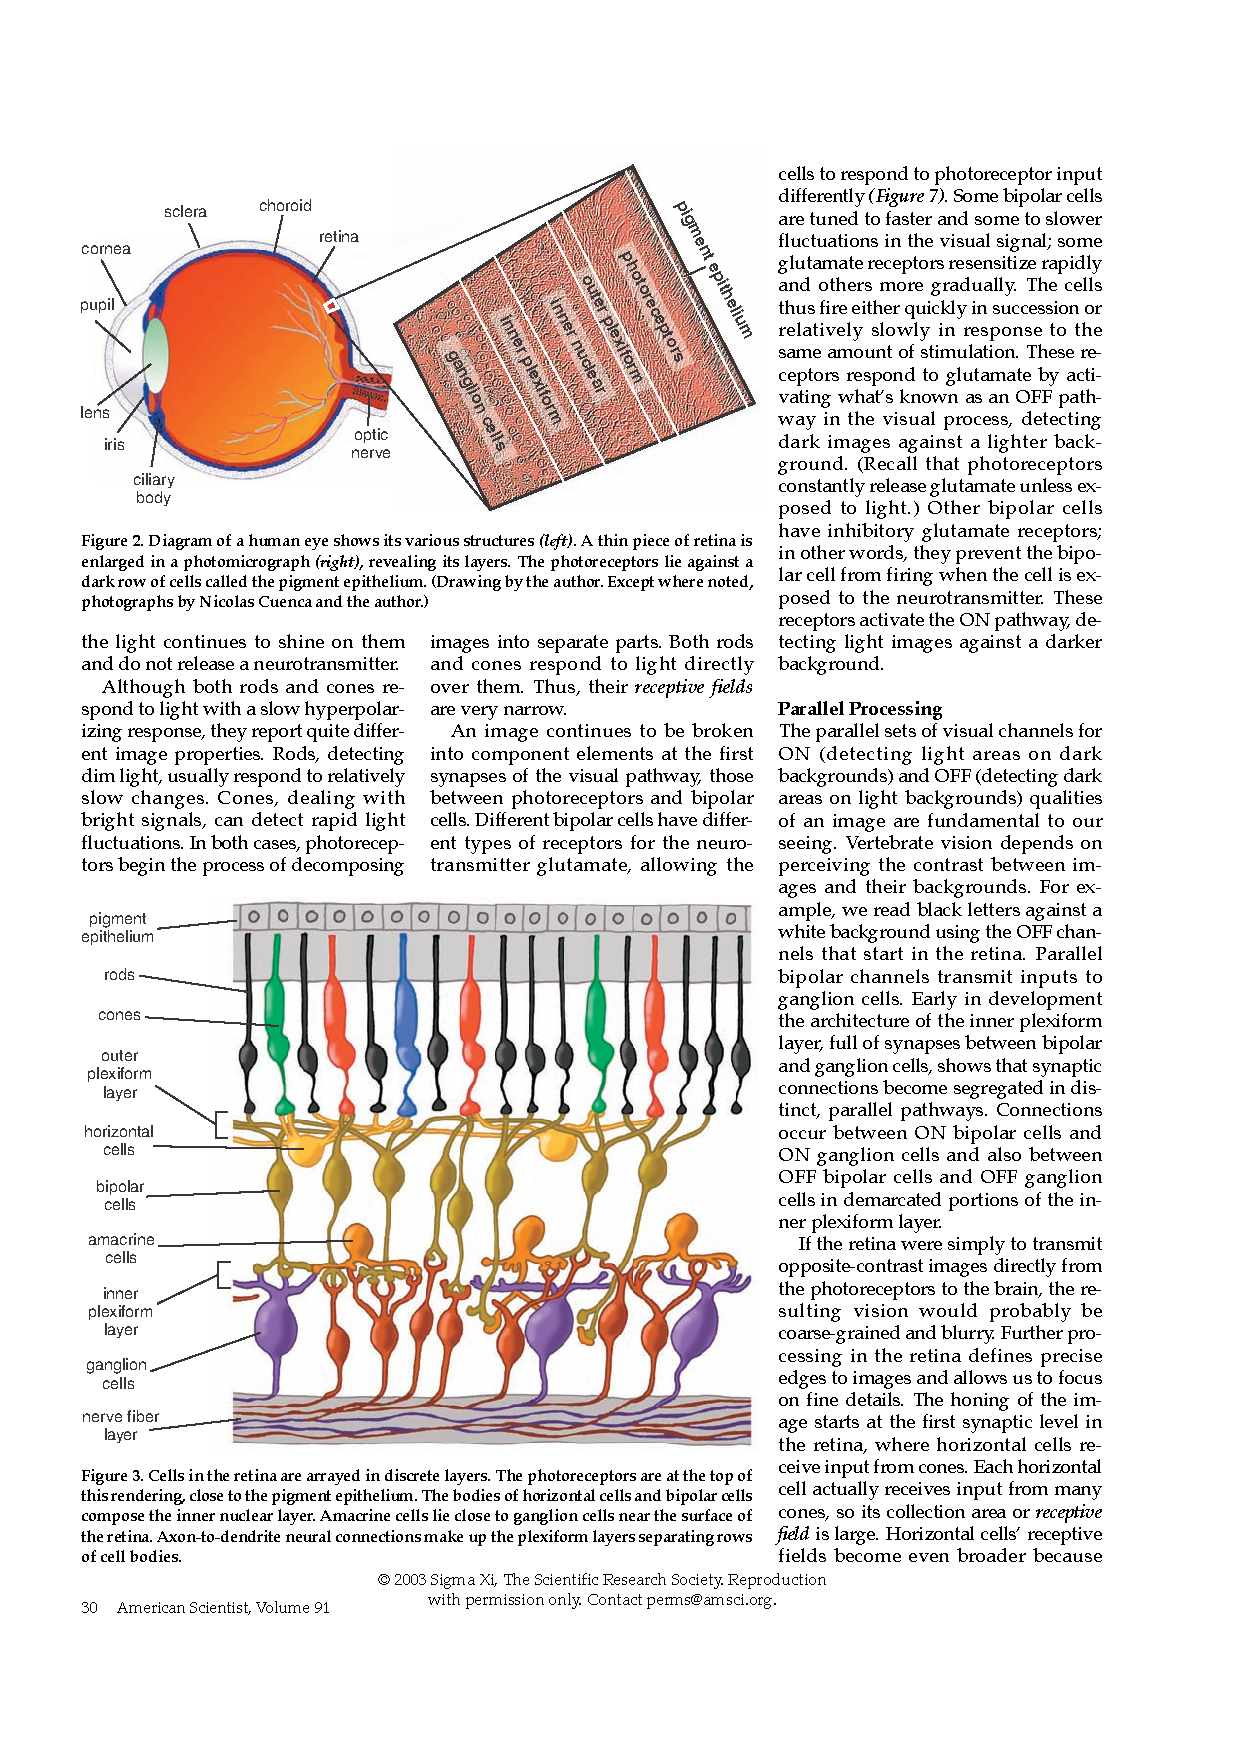
\includegraphics[width=0.8\textwidth, trim=1cm 21cm 8cm 2.5cm, clip]{images/kolb-2003-howtheretinaworks-p3.pdf}
			\caption{Cross section of the human eye \citep{kolb2003retina}}
		\end{figure}

		- foeva centralis with high density of cells
		
		- blind spot where all nerve fibers leave the eye

		- fact: photoreceptors are on the "wrong" side of the retina

>--- cut
		-layers:
			- cons and rods: photo receptors
			- horizontal connections
			- bipolar cells
			- inner nuclear layer
			- inner plexiform layer: high density of dentrites from ganglion layer, cells with various functions (> 20), 
			- ganglion cells: generate action potential for encoded signals
<---
		
		- layers (information flow):
			- photoreceptors: cons and rods
			- outer plexiform: output of photoreceptors
			- inner nuclear: bipolar- (on, off), horizontal-, amakrine cells
			- inner plexiform: dentrites of the ganglion cells and axons of the inner nuclear cells (organized in layers)
			- ganglion cells generate action potential for encoded signals
			-optic nerve: about 1 million axons
		
		\begin{figure}[H]
			\centering
			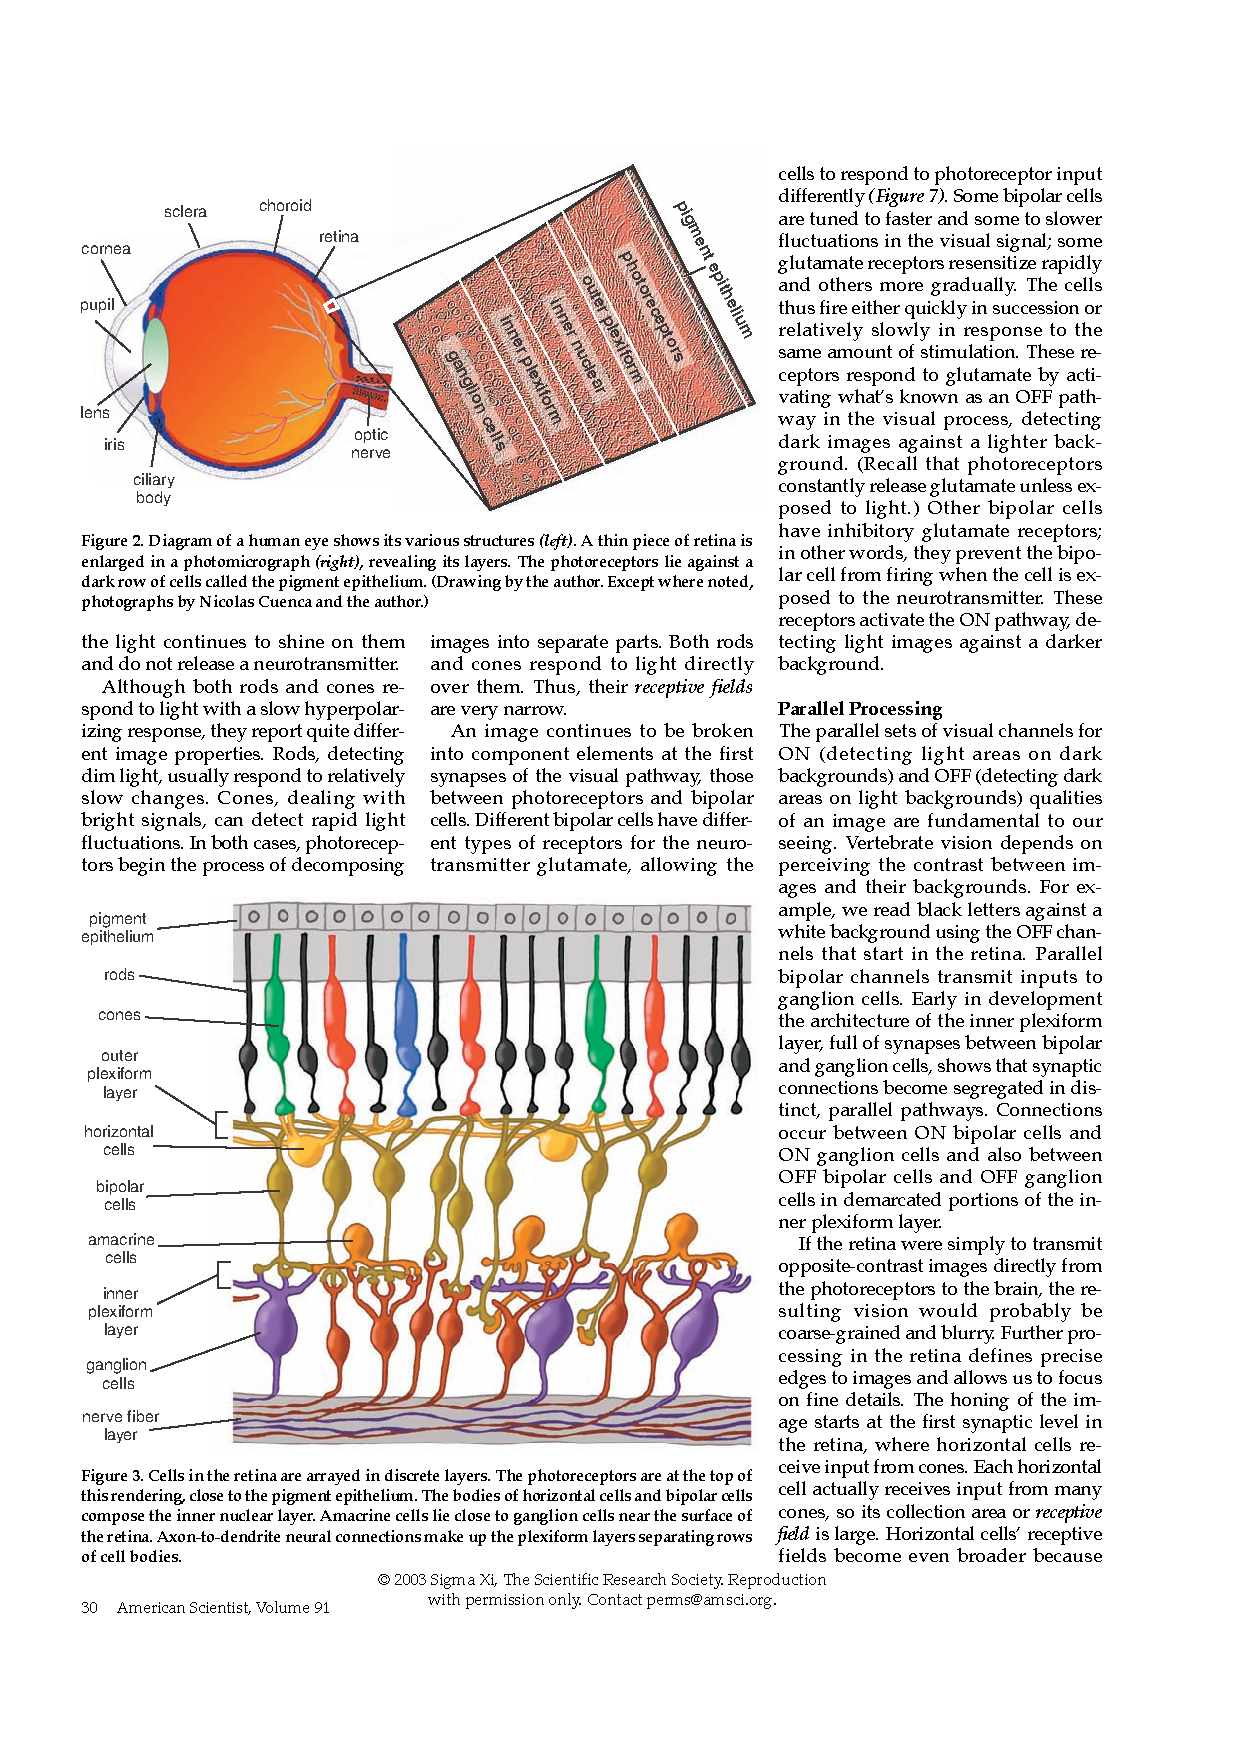
\includegraphics[width=0.5\textwidth, trim=1cm 5cm 8cm 15cm, clip]{images/kolb-2003-howtheretinaworks-p3.pdf}
			\caption{Cross section of the retina \citep{kolb2003retina}}
		\end{figure}
		
		- special function cells > new type of cell for each function
		
		\begin{figure}[H]
			\centering
			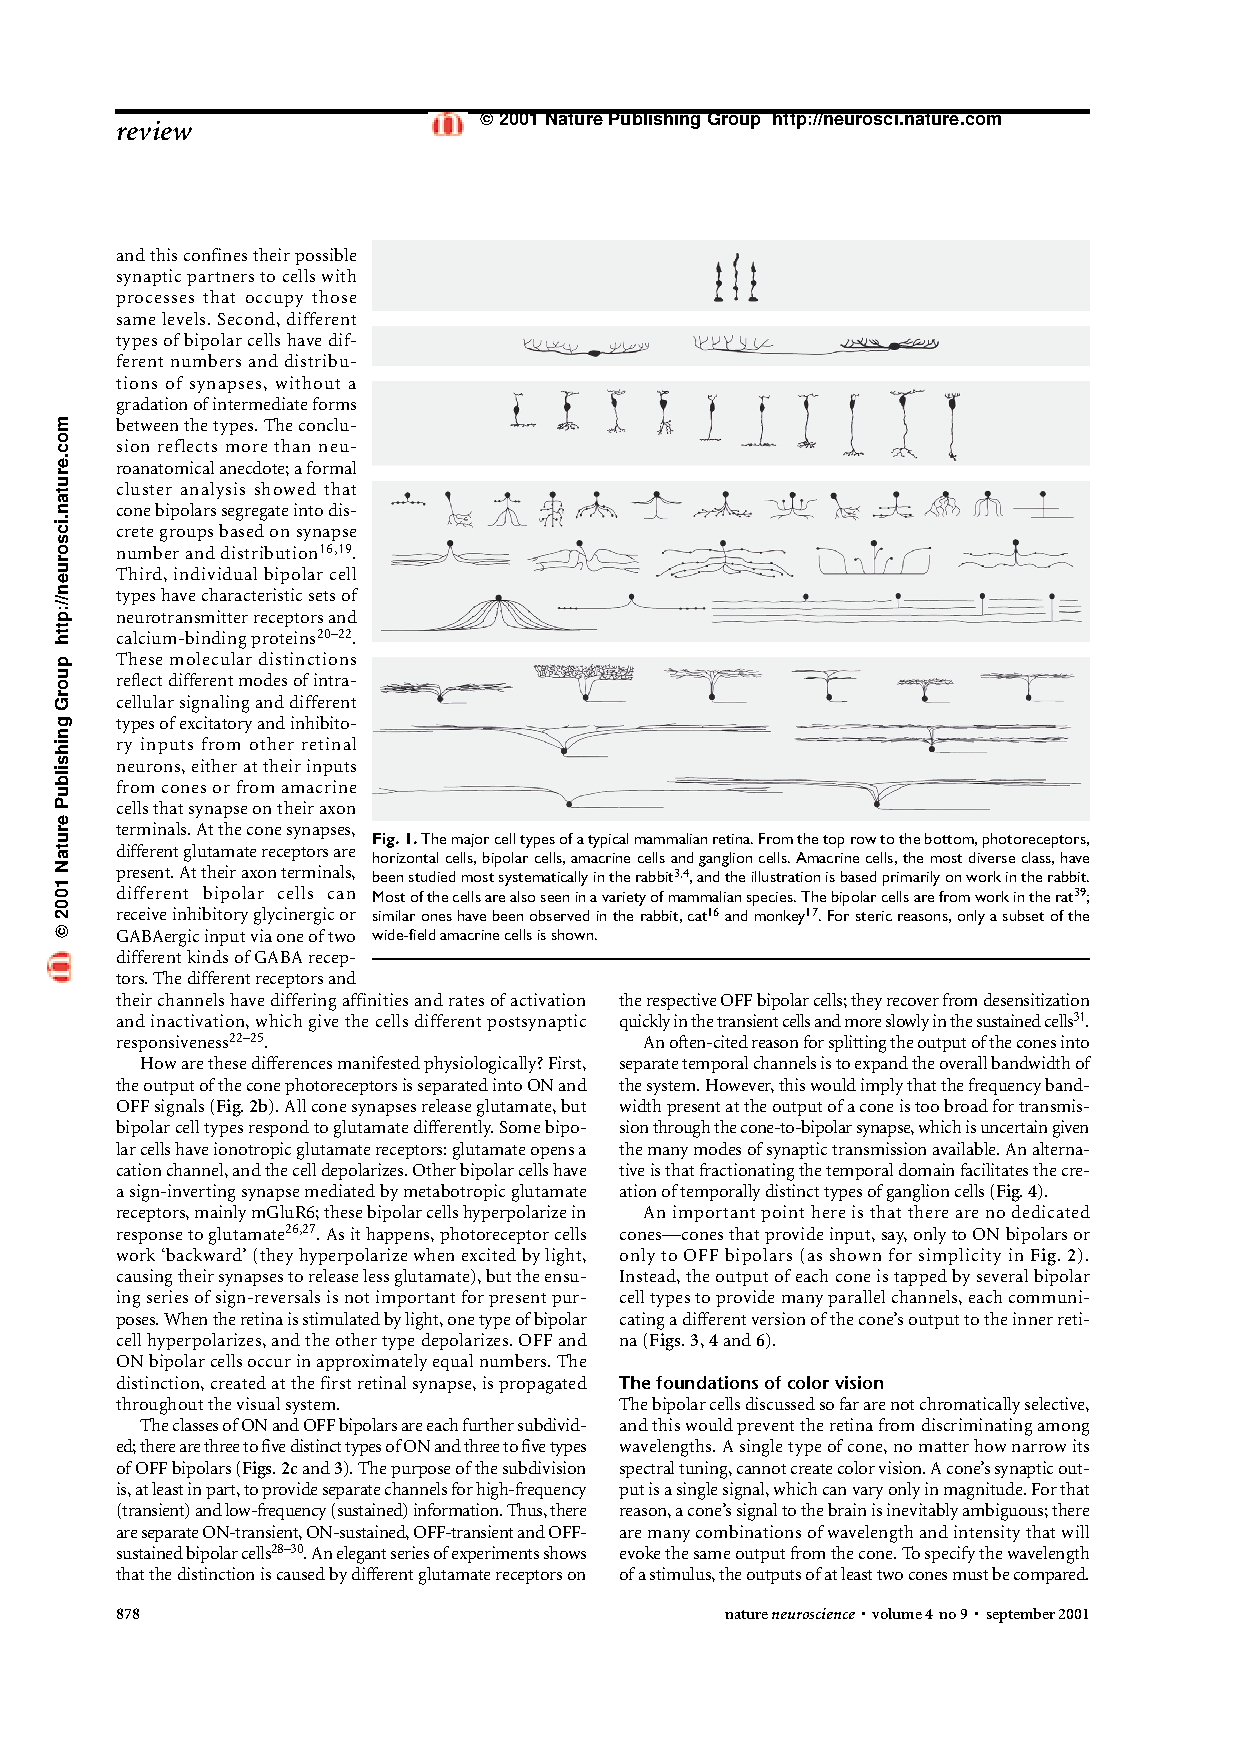
\includegraphics[width=\textwidth, trim=6.2cm 15.7cm 2cm 4cm, clip]{images/masland-2001-neuron-types.pdf}
			\caption{Different types of neuroes in the layers of the retina \citep{masland2001fundamental}}
		\end{figure}
		
		output:
			- mainly to the LGN and from then on in the primary visual cortex
			- other low level functions: pupil control, shut lids on flash, ...
		
		output characteristics:
			- everything happens in parallel
			
		special low level function:
			- inhibit signals caused by eye or head movement (object motion sensitive cells)

	\section{Lateral geniculate nucleus}
	
		- information from retinal ganglion cells
	
		- keep short
	
	\section{Visual cortex}

		- brain regions that are responsible for evaluation, analysis

		\begin{figure}[H]
			\centering
			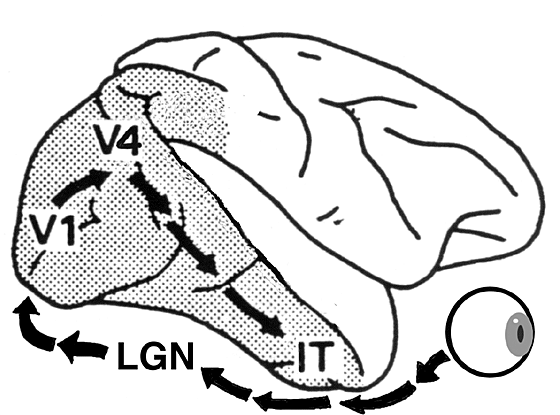
\includegraphics[width=0.5\textwidth]{images/riesenhuber-poggio-2000-visualpathway.png}
			\caption{Locations of the different visual cortices}
		\end{figure}
		
		- IT as highest level region near hippocampus, memory

		\begin{figure}[H]
			\centering
			\captionsetup{justification=centering,margin=2cm}
			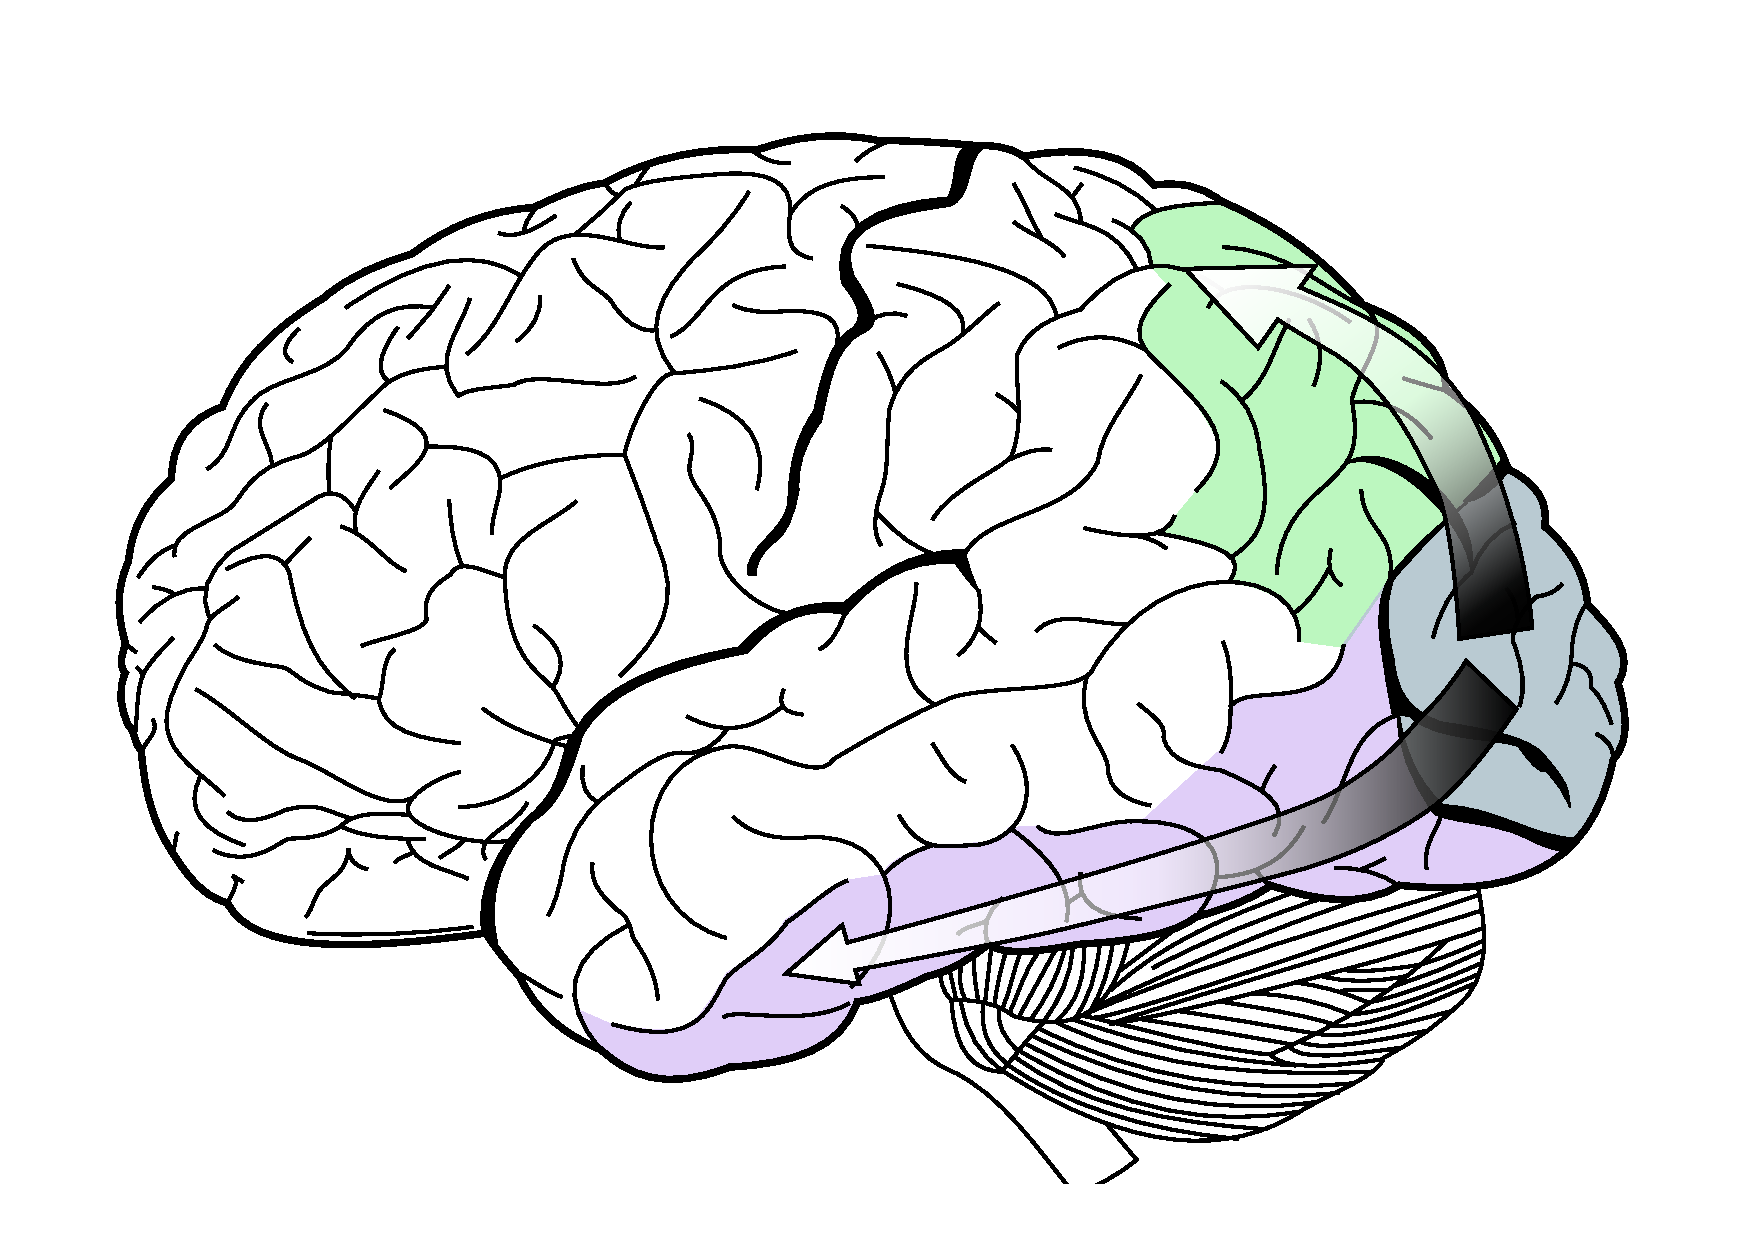
\includegraphics[width=0.7\textwidth]{images/visual-stream2.pdf}
			\caption{Ventral (purple) stream going to temporal lobe and dorsal (green) stream heading to parietal lobe}
		\end{figure}
		
		- V1 (striate cortex) early vision
		
		- V2-V4, IT (extra-striate areas)
		
		- ventral stream: V1 - V2 - V4 - IT
			- recognition functions
			- focused on information from foeva centralis
			- consciousness
		
		- dorsal stream: V1 - V2 - The parietal lobe is one of the four major lobes of the cerebral cortex in the brain of mammals.
			- subconsciousness
			- all retina information
			- high frequency processing > i.e. motion
	
\chapter{Biologically Inspired Computational Models of the Visual System}

	- most accurate model would simulate molecular behavior but this is to complicated
	
	\section{Types of Models}
		
		- start to abstract functional entities
			- first model a neuron
			- second model a bunch of neurons (functional areas)
		
		\subsection{Numerical Simulations}
		
			- simulating single neurons
		
			- very impractical because of high computational efforts, slow
		
		\subsection{Functional Models}

			bottom-up vs top-down
			
			- stimulus-driven: characteristics like luminance, contrast, ...
			
			- top-down (goal driven): viewing task, expectations based on other stimuli or memory, temporal continuity, reasoning (visual attention)
	
		
	\section{Signal Propagation}
	
		- Retina is simple, one-way connection only
		
		- LGN
	
		\subsection{Feed-Forward only}
		
			- It is assumed that the first ~150 ms are feed-forward only. \cite{thorpe1996speed}
			
			- Many models that limit them to this > fast recognition tasks
			
			- very good results with same performance as traditional approaches

			\begin{figure}[H]
				\centering
				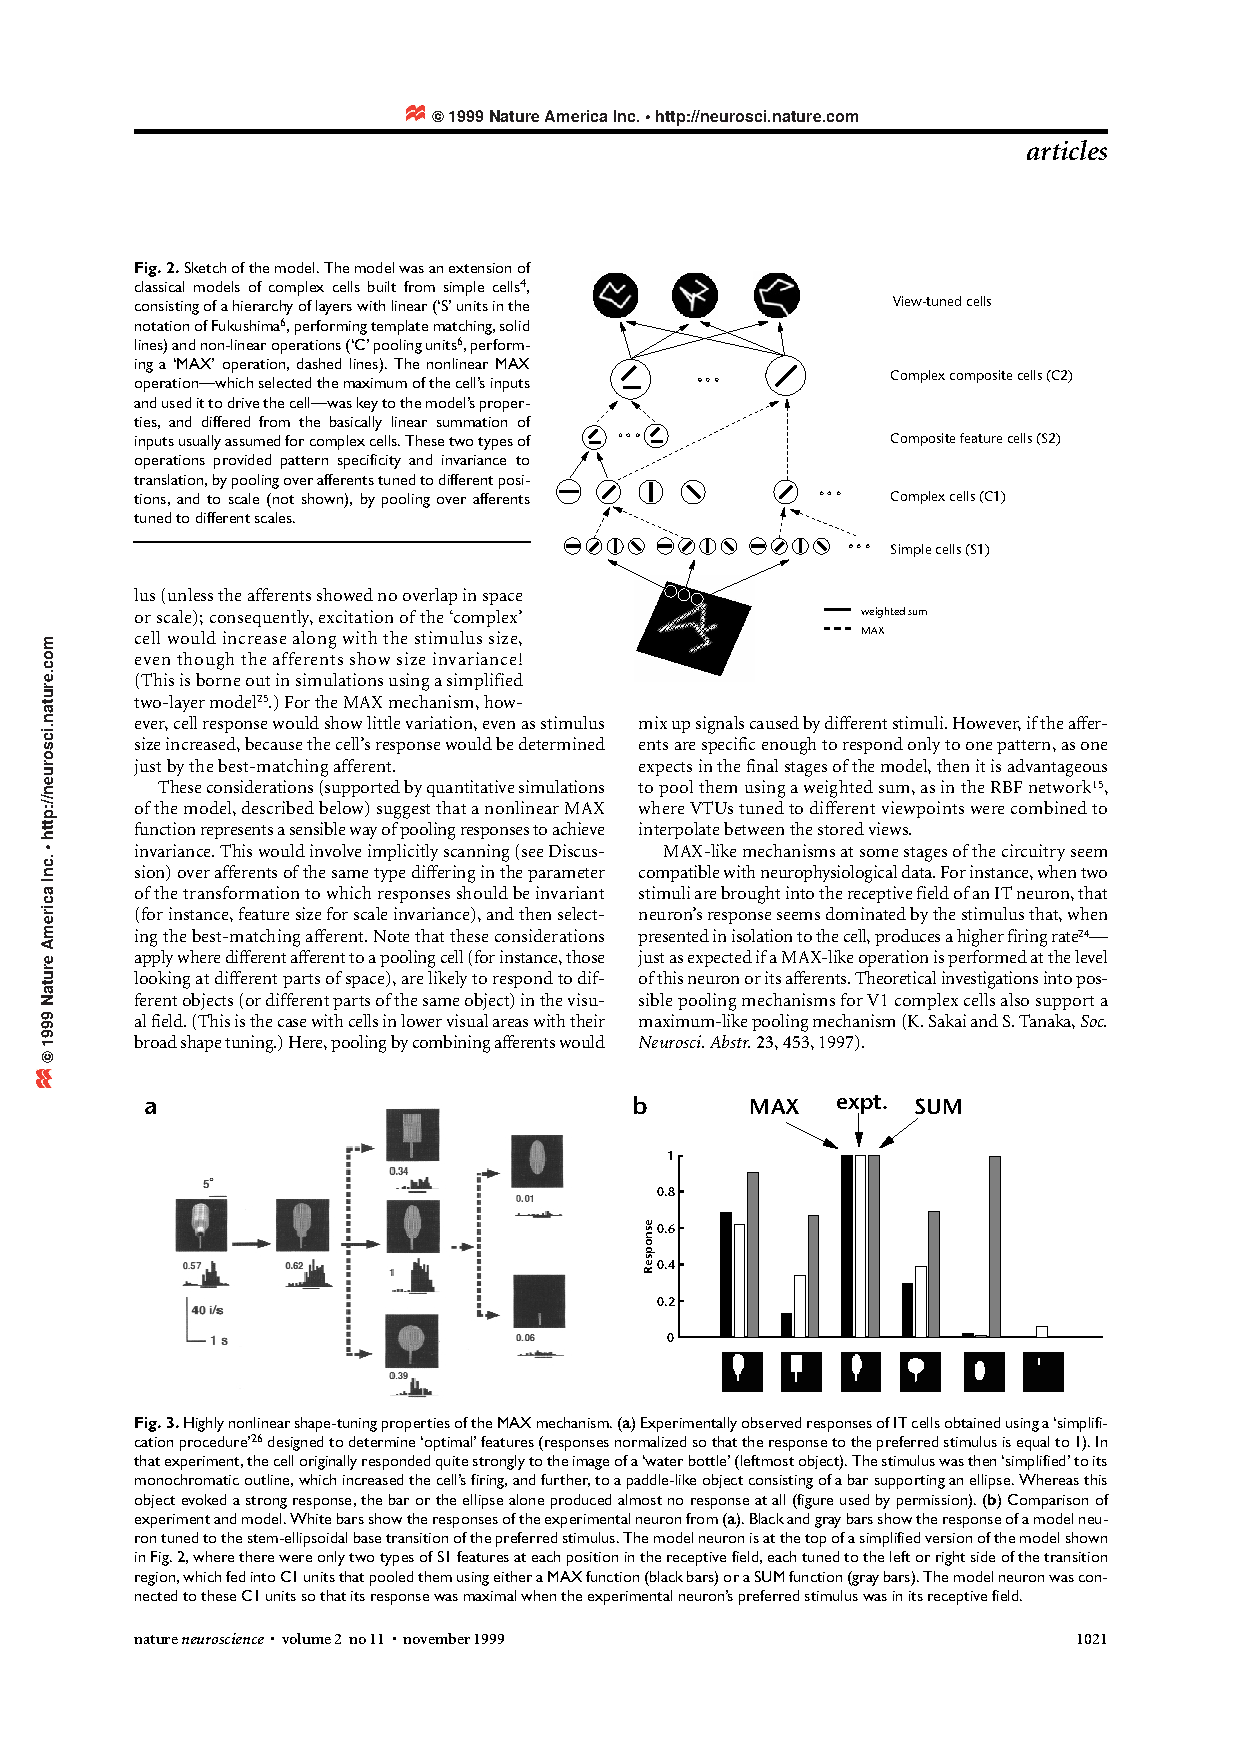
\includegraphics[width=0.8\textwidth, trim= 9cm 18cm 2.5cm 4cm, clip]{images/riesenhuber-poggio-1999-models-p3.pdf}
				\caption{Model of V1 to IT \citep{riesenhuber1999hierarchical}}
			\end{figure}
		
		\subsection{Recurrent: Feed-Forward and Feedback}
		
			- Why is it important to consider feedback (= visual attention)?
			
			- Saliency > i.e. for landmark recognition moving objects should be ignored, search for prominent object in image
			
	\section{Examples for models}
	
		\subsection{Only Feed-Forward model i.e. by Serre et al.}
		
			- simple and complex cells by hubel and wiesel
		
			- HMAX, Riesenhuber, Poggio extended this to object recognition
		
			- + feature learning at higher levels: Serre et al., Robust Object Recognition with Cortex-Like Mechanisms, 2007
			
		\subsection{Supervised Learning}
		
			- ...
		
		\subsection{Biological plausibility}
		
			- no feedback
			
			- needs many examples for learning an object
			
			- clutter in scene causes big issues
			
			> Problems may be solved using feedback

			- include this hierarchy image

		\subsection{Comparison with State-of-the-Art Artificial Object Recognition}
		
			- common test framework: Caltec101
		
			- regarding categorization
 
\chapter{Application: Localization}

	- first, object recognition
	
	- second, location of the objects must be known
	
	- third, different information pieces must be put together for exact localization (particle filter)


\chapter{Conclusion}

	still artificial RGB images are used, event based cameras are more biological accurate
	
